%HEADER:
\documentclass{article}
\usepackage[UTF8]{ctex}%Chinese supporting
\usepackage{xcolor}%colors.
\usepackage{amsmath}%math fonts
\usepackage{amssymb}%math symbols
\usepackage{luatexja-ruby}%nihon kanji +rubi+
\usepackage[normalem]{ulem}%improved underlines
\usepackage{graphicx}%pictures
\usepackage[colorlinks,linkcolor=red]{hyperref}%hyperlinks
\usepackage{multirow}%form
\usepackage{multicol}%form
\usepackage{makecell}%form
\usepackage{minted}%code environment
\usepackage[amsmath,thmmarks]{ntheorem}%theorem environment
\usepackage{datetime2}

%DEFINE VERSION:


%Limitation:
% There MUST be a space after Proofs!!!
% Compile 3 Times Needed!!!
% Define fonts for nihon characters, and change the fonts for them.

% NEW FUNCTION DEFINATION:
\newcommand{\DeclareCJKFont}[2]{\setCJKfamilyfont{#1}{#2}}
% Argument #1: ShortName, Argument #2: FontName;
\newcommand{\CreateShortcutForCJKFont}[2]{\newcommand*{#1}[1]{{\CJKfamily{#2}##1}}}
% Argument #1: CommandName, Argument #2: ShortName;
% Example:
% 1. \DeclareCJKFont{stsong}{SimSun} SimSun was declared as stsong.
% 2. \CreateShortcut{\songtizi}{stsong} Use \songtizi{...} to typeset words in SimSun.
\newcommand{\mr}[2]{\multirow{#1}{*}{#2}}
% Define Shortcut for \multirow command.

% VERSION CONTROL:
% USE `ver.lua' script to print version.
\newcommand{\ver}{\directlua{dofile('./ver/ver.lua')}}
% DEFINE \bumprevsi TO BUMP THE REVISION VERSION:
\newcommand{\bumprevis}{\directlua{dofile('./ver/bumprevis.lua')}}
\newcommand{\bumpminor}{\directlua{dofile('./ver/bumpminor.lua')}}
\newcommand{\bumpmajor}{\directlua{dofile('./ver/bumpmajor.lua')}}

% REDEFINE paragraph & subparagraph ENVIRONMENT:
\makeatletter
\renewcommand\paragraph{\@startsection{paragraph}{4}{\z@}%
{3.25ex \@plus1ex \@minus.2ex}%
{1.5ex \@plus.2ex}%
{\normalfont\normalsize\bfseries}}
\renewcommand\subparagraph{\@startsection{subparagraph}{5}{\z@}%
{3.25ex \@plus1ex \@minus.2ex}%
{1.5ex \@plus.2ex}%
{\normalfont\normalsize\bfseries}}
\makeatother

% NEW THEOREM ENVIRONMENTS DEFINATION:
\newtheorem{example}{例题}[subsection]
\newtheorem{definition}{定义}[subsection]
\newtheorem{thm}{定理}[subsection]
\theoremstyle{nonumberplain}
\theoremseparator{ }
\theoremheaderfont{\bf}
\theorembodyfont{\normalfont}
\theoremsymbol{\rule{1ex}{1ex}}
\newtheorem{Proof}{证明}
\newtheorem{solve}{解法}

% NOTES:
\newcommand{\note}{\ \par
	\subsection*{课堂笔记\\\tiny{Note on the text}}
	\newpage}

% PRESETs for minted, Contents, CTeX, picutures folders:
\setminted[C++]{autogobble,breaklines,frame=lines,fontsize=\footnotesize,mathescape}
\setminted[text]
{autogobble,breaklines,frame=single,fontsize=\footnotesize,mathescape}
\ctexset{punct={kaiming},linestretch={2}}
\graphicspath{{./pictures/}}
\setcounter{secnumdepth}{4}
\setcounter{tocdepth}{4}

% FONTS DECLARATION:

%%%%%%%%%%%%%%%%%%%


%DOCUMENT BEGINS:
\begin{document}
\bumprevis
\title{\Huge 动态规划入门\\\Large Dynamic Programming Book for Beginners\\
\author{Mingqi\_H\ and\ wcz}\date{\emph{version = \ver\\branch = 1.0}Build Time: \DTMnow}}
\maketitle

\thispagestyle{empty}%Disable Page Numbering for title page.
\pagestyle{empty}%Disable Page Numbering temporarily.

\ \\
\ \\
\ \\
\newpage
\ \\\ \\
\begin{center}\em{\large{To Hatsune Miku}}\end{center}
\newpage
\tableofcontents
\newpage

\pagestyle{plain}%Enable Page numbering.
\setcounter{page}{1}
\setcounter{section}{-1}

\section{自我介绍,前言}
\subsection{作者介绍}
本人黄铭祺,GRYZ三校区60级蒟蒻$OIer\times 1$.

参加过NOIp 2017提高组复赛.

我不会DP,但是既然老师要我讲,那也就现学现卖地来讲一点.

 另外我不会讲课,很有可能讲不好,如果有错误还请指出。
\subsection{参与者}
	参与文档改进的是同一学校的另一位 wcz 同学.wcz 本人与作者是好朋友.

\subsection{前言}
这篇文章主要介绍动态规划,当然动态规划是一种思想,题目种类也非常多,不可能在这么短的时间内讲完,所以这节课主要是对动态规划的初步介绍,会做最基础的题目,更重要的是理解动态规划的思想,这就足够了。

当然,需要有一定的前置知识,即语言部分与图论,搜索,这里默认读者们拥有一定的编程经验和对基本算法有一定的了解。

这节课要讲的东西可能有些多了。大家先看看目录讨论一下重点要听什么内容。序列型DP、背包问题是所有DP的基础,棋盘型DP、区间型DP什么的也要涉及一点,剩下的类型就看讲课的时间和大家的理解程度吧。

这节课覆盖的内容有几乎所有常见种类的DP,以及DP优化的一些技巧,是为了让各位对DP的各种类型有一个初步的了解。各个例题应该都属于非常基础的类型,如果搞不懂的话可以上网查相关资料。


\newpage

\section{对动态规划的初步了解}
动态规划通常是用来处理一些最优化问题, 需要问题具有可以划分阶段的特性以及其抽象模型所需要满足的一些条件.
可以将对问题一定阶段的解法抽象成一个状态, 从这一阶段的状态得到下一阶段的状态的过程被称为状态转移, 我们的目标就是求出完整问题的最优状态.
\subsection{一些定义}
\begin{definition}[状态]
	状态是指解决问题过程中的每个步骤或可能,类似搜索中的状态(还记得搜索题常见的cur和nxt这两个变量吗?就是这样的东西)。
\end{definition}
\begin{definition}[状态转移方程]
	状态转移方程是指解决问题过程中,由步骤$A$到步骤$B$所需要进行的操作以及状态发生的变化,类似搜索中状态的扩展(还记着八皇后问题中dx和dy这两个数组吗?就是类似这样的东西,实际上就是从上一步到这一步所需要进行的操作或者什么东西的改变)。
\end{definition}

\subsection{动态规划实例}
我们先来看一道题目:

\begin{example}由正实数构成的数字三角形排列如图所示,第一行的数为$a_{11}$;第二行的数从右到左依次为$a_{21},a_{22},\cdots$.第$n$行的数为$a_{n1},a_{n2},\cdots,a_{nn}$。从$a_{11}$开始,每一行的数$a_{ij}$只有两条边可以分别通向下一行的两个数$a_{(i+1)j}$和$a_{(i+1)(j+1)}$。用动态规划算法找出一条从$a_{11}$向下通到$a_{n1},a_{n2},\cdots,a_{nn}$中某个数的路径,使得该路径上的数之和达到最大.

	令$f(i,j)$是从$a_{11}$到$a_{ij}$路径上的数的最大和,并且$f(i,0)=f(0,j)=0$,则$f(i,j)=(\ \ \ )$.
	\begin{center}
		\begin{math}
			\begin{matrix}
				&a_{11}&         \\
				&a_{21}&\ a_{22}         \\
				&a_{31}&\ a_{32}&\ a_{33} \\
				&\vdots&\vdots&\vdots&       \\
				&a_{n1}&\ a_{n2}&\ \cdots&\ a_{nn}
			\end{matrix}
		\end{math}
	\end{center}

	\ \ A.\ $\max_\{f(i-1,j-1),f(i-1,j)\}+a_{ij}$

	\ \ B.\ $f(i-1,j-1)+f(i-1,j)$

	\ \ C.\ $\max\{f(i-1,j-1),f(i-1,j)\}$

	\ \ D.\ $\max\{f(i,j-1),f(i-1,j)\}+a_{ij}$
\end{example}

题目中涉及的$f(i,j)$其实就是一个可行的\textbf{状态设计}, 状态设计所必须满足的条件是它包含着所有需要的信息, 对例题来说只需要知道此到达位置的\textbf{最大收益}而无需知道\textbf{具体路径}.

这道题就是NOIp 2017提高组初赛试题第11题,一个经典的数字三角形问题。但是已经涉及到了动态规划的本质了。动态规划最重要的两步就是\textbf{设计状态}和考虑\textbf{状态转移方程}。
以上内容涉及到两个非常重要的概念,状态和状态转移方程。我们先不学习DP,而是先温习一下我们已经\textbf{具备的知识}。

同学们大概是会做基本的递推和搜索了.

大部分动态规划都可以被表示成一种递推的形式.

对于搜索,fDP就可以看成是一种搜索。本质与搜索并没有任何不同,那么为什么搜索的时间复杂度会达到$O(2^n)$,而DP可以做到$O(n^k)$的时间复杂度呢?

大家应该知道,搜索是利用状态转移来完成问题的整个步骤的,动态规划也是这么做的,我认为它与搜索的最本质区别是它是利用上一步的最优状态来进行这一步的转移.而搜索是利用上一步的所有状态来进行本步的转移并且在其中选择最优的那个来更新答案.

这就可以看出,动态规划能做的事情搜索都是能做的.但是有搜索能做但是动态规划不能做的.

什么时候动态规划能解决这个问题呢?问题关键是"最优"两个字.
这里会涉及到做动态规划的两个前提: \textbf{最优子结构} 和 \textbf{无后效性} .


\subsubsection{最优子结构}尝试从直观上去体会它的含义.

对于一个可以划分为若干阶段的问题.如果能利用它的一个\textbf{子问题的最优解}得到\textbf{整个问题的最优解}.那么这个问题是具有最优子结构的.

对于这个问题,从起点出发到达终点的最优解是整个问题的解,而从起点到达其中不是终点的某个点的最优解是整个问题一个子问题的解.

考虑这个例题具不具有最优子结构.
我们可以发现,如果最终的最优解出现在$f(u,v)$,也就是从起点以某条路径走到$f(u,v)$会获得最大收益.

考虑到达$(u,v)$的路径,我们知道只有两个点能到达$(u,v)$,也就是$(u-1,v-1)$和$(u-1,v)$,那么容易知道问题的最优解一定是从这两个点的最优解转移过来的.不然一定会有更优的解.
说明这道例题是具有最优子结构的.
所以通过求出$f(u,v-1)$和$f(u-1,v-1)$就可以得到$f(u,v)$.




\subsubsection{无后效性}
无后效性指的是问题的一个阶段的状态已知,那么这个阶段此后的阶段只与此阶段有关,而与之前发生过的所有阶段的状态无关,也不会影响到未来的任何阶段.
对于例题,从起点到达某个点$(u,v)$的最大收益需要通过$f(u-1,v)$和$f(u-1,v-1)$来求解,而不需要知道$f(u-2,v-1)$或者再之前的状态.状态$f(u,v)$也不会影响到$f(u-2,v-1)$等未来的状态.
我们知道例题同样是满足无后效性的.

通过对问题的进一步学习我们会知道对于一个问题的无后效性取决于\textbf{状态设计}.


\begin{solve}
	通过对问题的进一步分析容易得到问题的解法.
	其状态转移方程可以这么写:
	\begin{equation*}
		f(i,j)=\max\{f(i-1,j),f(i-1,j-1)\}+a_{ij}
	\end{equation*}
	根据在递推方面的经验我们可以如果需要求出最终结果$f(u,v)$.
	我们首先需要求出$f(u-1,v-1), f(u-1,v)$ .
	如果一步一步逆推的话, 大概需要递归来解决.
	我们大概需要在程序中设计一个函数$f(i,j)$.
\begin{minted}{C++}
f(i,j)
return max{f(i-1,j),f(i-1,j-1)}+a(i,j)

ans()
return f(u,v)
\end{minted}
而对于这个问题而言正推和逆推并没有本质区别.

按照递推的设计思路, 这个程序应该这样设计.
\begin{minted}{C++}
for(int i=1;i<=u;++i)
	for(int j=1;j<=v;++j)
		f[i][j]=max(f[i-1][j]+f[i-1][j-1])+a[i][j];
\end{minted}
\end{solve}
\subsection{动态规划的应用及其局限性}
大家应该提高对于动态规划的重视.
在NOIp中,动态规划通常会出1~2个题目, 当然并不是所有人都能全部做出来的, 说它没用,是因为如果不能想出可靠的转移, 反而浪费了大量的时间, 还不如写最简单的算法, 并且NOIp通常情况下会给不少的部分分,这部分部分分通常用不到60行代码就能拿到, 这意味着我们学好暴力,每道DP题就可以拿到20~60分。

动态规划当然不是万能的, 有很大的\textbf{局限性}, 这一点在前面有所介绍.
\begin{itemize}
	\item{所解决的问题必须是满足\textbf{最优子结构}和\textbf{无后效性}的textbf{可分阶段}的问题.}
	\item{某些能用动态规划解决的问题可能会有其他更好更优的算法.}
	\item{其本身的局限性, $n^k$的时间复杂度以及同样规模的空间占用.}
	\item{设计出足够优秀的状态这有时是很难的, 见多识广很重要.}
\end{itemize}
\textcolor{white}{希望大家不要放弃,OIer这个群体很是特殊,并且饱受排挤,大家一定坚持下去,不管外界怎么看待我们,一定要记住自己的目标。不忘初心,方得始终。}

\section{动态规划基础------序列型DP}
应某位dalao要求,在讲今天的主要内容之前,先讲一下最基础的序列型DP,即最长子序列问题。
\subsection{最长上升子序列问题---LIS}
\subsubsection{介绍与实现}
\begin{definition}[最长上升子序列]
	给出一个序列$a_1, a_2, \cdots, a_n$,求它的一个子序列(设为$s_1, s_2, \cdots, s_n$),使得这个子序列满足这样的性质:$s_1<s_2<s_3<\cdots<s_n$并且这个子序列的长度最长。输出这个最长的长度。
\end{definition}

以上是最长上升子序列的定义。其他最长子序列问题的定义也类似。



考虑状态dp[i]表示当前枚举到了第i个数,当前最长上升子序列长度为dp[i]。

用arr[]表示原数组,dp[]表示最长上升子序列的长度。我们枚举每一个数,每一个数都枚举其前面所有的数。如果当前枚举到的数大于之前枚举的数,那么最长上升子序列的长度一定至少比这个大1(为什么?)。用一个ans变量暂存一下,然后枚举结束后用ans更新一下当前的最长上升子序列的长度即可。
\begin{minted}{C++}
int ans;  
dp[1] = 1;  
for(int i = 2; i <= n; ++i)  
{
    ans = dp[i];  
    for(int j = 1; j < i; ++j)
        if(arr[i] > arr[j] && dp[j] > ans)  
            ans = max(ans, dp[j]);  
    dp[i] = ans + 1;
}
\end{minted}

时间复杂度$O(n^2)$。

当然这不是最优化的方法,考虑一下如何优化?

明显的,我们可以看到第二层枚举不是必需的。第二层枚举的作用是找到最接近且比当前枚举的数。所以可以使用二分查找优化掉这一层循环。

增加一个b数组,b[i]用以表示长度为i最长子序列的最后一个数最小可以是多少,k表示当前b数组的长度,则:

\begin{equation*}
	dp[i]=\begin{cases}
		b[k+1]=arr[i]                  & , arr[i]>b[k] \\
		b[binary\_search(arr[i],1,k)] & , arr[i]<b[k]
	\end{cases}
\end{equation*}

容易发现,b数组始终是单调递增的。所以我们可以二分查找arr[i]在b数组出现的位置,从而把时间复杂度降至$O(n\log n)$。

二分应该都会吧?如果不会二分的话就看看代码:

\begin{minted}{C++}
int binarySearch(const int *Array,int start,int end,int key)
//Array:待查找的数组,start:起始点下标,end:终止点下标,key:待查找的数。
{
    int left,right;
    int mid;
    left=start;
    right=end;
    while(left<=right)
    {
        mid=(left+right)/2;
        if(key==Array[mid])  return mid;
        else if(key<Array[mid]) right=mid-1;
        else if(key>Array[mid]) left=mid+1;    
     }
     return -1;//没有找到
}
\end{minted}

以上二分代码适用于一般情况,更常用的写法:
\begin{minted}{C++}
int binarySearch(int num, int l, int r)
//num为待查找的数。
{    
    while(l <= r)    
    {    
        int mid = (l+r)/2;    
        if(num >= b[mid])    
            l = mid + 1;    
        else  
            r = mid - 1;    
    }    
    return l;
}
\end{minted}

当然如果愿意用STL的话,lower\_bound()函数也很好用:

\begin{minted}{C++}
#include<algorithm>
std::lower_bound(first,last,val);//在区间[first,last)中二分查找元素val。
//如果找到相应的val,则返回一个指向元素位置的指针;
//否则返回一个指向最接近val且小于val的元素位置的指针。
//另外一种用法:
std::lower_bound(first,last,val,comp);
//以自定义comp作为比较器进行比较(类似sort的用法),返回值同上。
//同理还有upper_bound()函数。
\end{minted}
\subsubsection{LIS的打印}
在状态转移的时候记录一波转移方向,保存在pre[]数组中,然后需要输出的时候就可以根据pre[]数组逆序构造出LIS,使用一个栈保存起来就可以正向输出了。

代码实现起来比较容易,自己写一下,也不那么常用。
\subsubsection{例题---导弹拦截}
\begin{example}导弹拦截\\
	\textbf{题目描述}

	某国为了防御敌国的导弹袭击,发展出一种导弹拦截系统。但是这种导弹拦截系统有一个缺陷:虽然它的第一发炮弹能够到达任意的高度,但是以后每一发炮弹都不能高于前一发的高度。某天,雷达捕捉到敌国的导弹来袭。由于该系统还在试用阶段,所以只有一套系统,因此有可能不能拦截所有的导弹。

	输入导弹依次飞来的高度(雷达给出的高度数据是不大于50000的正整数),计算这套系统最多能拦截多少导弹,如果要拦截所有导弹最少要配备多少套这种导弹拦截系统。\\
	\textbf{输入输出格式}
	\ \\
	\textbf{输入格式:}

	一行,若干个整数(个数少于100000)
	\ \\
	\textbf{输出格式:}

	2行,每行一个整数,第一个数字表示这套系统最多能拦截多少导弹,第二个数字表示如果要拦截所有导弹最少要配备多少套这种导弹拦截系统。
	\ \\
	\textbf{输入输出样例}
	\ \\
	\textbf{输入样例:}
	\begin{minted}{text}
389 207 155 300 299 170 158 65
\end{minted}
	\textbf{输出样例:}
	\begin{minted}{text}
6
2
\end{minted}
\end{example}

导弹拦截这道题目出自NOIp 1999,容易看出第一问是一个裸的LIS问题(最长不升子序列就是LIS的一个变形而已)。可以直接套上LIS的板子看看能不能拿到100分。


\note
\subsection{最长公共子序列---LCS}
\subsubsection{介绍与实现}
\begin{definition}[最长公共子序列]
一个数列,如果分别是两个或多个已知数列的子序列,且是所有符合此条件序列中最长的,则称为已知序列的最长公共子序列。在计算机科学中,最长递增子序列是指,在一个给定的数值序列中,找到一个子序列,使得这个子序列元素的数值依次递增,并且这个子序列的长度尽可能地大。
\end{definition}

以上是对最长公共子序列问题的定义。理解一下。

考虑一下这种题目如何打暴力。

非常容易,对吧,就是暴力枚举第一个序列的每一个子序列,对每一个子序列判断它是否为第二个序列的子序列。然而这样的时间复杂度是$O(2^{\min(n,m)})$的,其中n, m为字符串的长度。

思考这样一个性质:如果一个LCS是另一个LCS的前缀,那么一定存在一个LCS,使得它的长度为这两个LCS长度之和。

\begin{thm}[LCS的最优子结构]
	令$X=\langle x_1, x_2, \cdots, x_m\rangle$和$Y=\langle y_1, y_2,$ $\cdots,y_n\rangle$为两个序列,$Z=\langle z_1, z_2, \cdots, z_k\rangle$为X和Y的任意LCS。
	\begin{enumerate}
		\item{如果$x_m=y_n$,则$z_k=x_m=y_n$。且$Z_{k-1}$是$X_{m-1}$和$Y_{n-1}$的一个LCS。}
		\item{如果$x_m\neq y_n$,那么$x_m\neq y_n$意味着$Z$是$X_{m-1}$和$Y$的一个LCS。}
		\item{如果$x_m\neq y_n$,那么$z_k\neq y_n$意味着$Z$是$X$和$Y_{n-1}$的一个LCS。}
	\end{enumerate}
\end{thm}

举个例子:
\begin{center}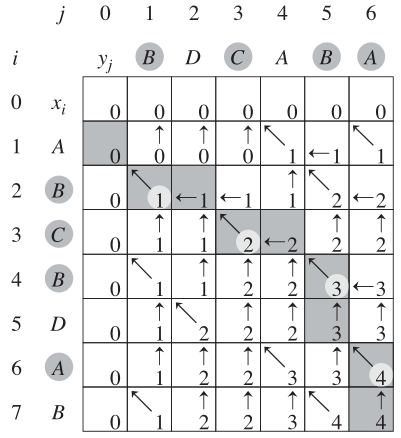
\includegraphics[height=5cm]{CLRS_LCS.png}\end{center}

上图是求$X=\langle A, B, C, D, B, D, A, B\rangle$和$B=\langle B, D, C, A, B, A\rangle$的LCS的过程。

\begin{Proof}
	(1)如果$z_k\neq x_m$,那么可以将$x_m=y_n$追加到$Z$的末尾,得到$X$和$Y$的一个长度为$k+1$的公共子序列。与$Z$是$X$和$Y$的最长公共子序列的假设矛盾。因此,必然有$z_k=x_m=y_n$。这样,前缀$Z_{k-1}$是$X_{m-1}$和$T_{n-1}$的一个长度为$k-1$的公共子序列。我们希望证明它是一个LCS。利用反证法,假设存在$X_{m-1}$和$Y_{n-1}$的一个长度大于$k-1$的公共子序列$W$,则将$x_m=y_n$追加到$W$的末尾会得到$X$和$Y$的一个长度大于$k$的公共子序列,矛盾。

	(2)如果$z_k\neq x_m$,那么$Z$是$X_{m-1}$和$Y$的一个公共子序列。如果存在$X_{m-1}$和Y的一个长度大于$k$的公共子序列$W$,那么$W$也是$X_m$和$Y$的公共子序列,与$Z$是$X$和$Y$的最长公共子序列的假设矛盾。

	(3)与情况(2)对称。\ 
\end{Proof}

于是我们get到了LCS的一个很重要的性质,没有后效性,具有最优子结构的性质。这是LCS问题可以DP的基础。

很容易看出,最初我们写的暴力求解算法中,有大量重叠的子问题(考虑求子序列$X = \langle x_a, x_{a+1}, \cdots, x_b\rangle$的LCS,必定求这个子序列的子序列$Y = \langle x_{a+m}, x_{a+m+1}, \cdots, x_{a+n}\rangle$这个子序列的LCS),所以LCS问题也有重叠子问题性质。

由上述定理我们就可以写出一个递归解。刚才的暴力中我们是枚举每一个子序列,然后进行判断,现在我们考虑能否直接构造出这样的一个序列。

明显的,状态转移有以下两种:
\begin{itemize}
	\item{如果两位相等,那么新的LCS可以连接到旧的LCS之后,构成一个新的较长的LCS。}
	\item{如果两位不相等,那么新的LCS不变,还是前一位的最长的LCS。}
\end{itemize}
设状态f[i][j]表示到字符串X的第i位与字符串Y的第j位的LCS长度,则:
\begin{equation*}
	f[i][j]=\begin{cases}
		f[i-1][j-1]+1             & , X[i]=Y[j]     \\
		\max(f[i][j-1],f[i-1][j]) & , X[i]\neq Y[j].
	\end{cases}
\end{equation*}

根据上面的状态转移方程写出代码即可,时间复杂度$O(nm)$.
\subsubsection{LCS的打印}
同LIS的打印,记录一下转移的方向,然后就可以了,时间复杂度为$O(nm)$。
\subsubsection{LCS的优化}
考虑一下是不是有什么地方还可以优化。

考虑上一节说的LCS的打印的过程,也可以不记录下转移的方向,因为每个状态转移的方向都是固定的,所以可以在$O(1)$的时间内判断出一个状态是由三个状态中的哪一个转移而来的,因此不再需要pre[]数组,只需要在输出过程中逆序转移,判断一下转移方向,把每一个数丢到栈里,再依次输出即可。

对于不需要输出LCS的问题,还可以使用滚动数组优化一下f数组的空间占用。因为每次转移只用到了f数组当前的一行以及前一行,所以只需要保留这两行数据即可。但是如果需要计算LCS的元素,就不能使用滚动数组优化(思考一下为什么)。

例题的话,可以参考一下洛谷P1439 的前50\%,至于后面的优化,建议参考一下题解,因为严格意义上这个优化意义不是很大,常数也很大,不是那么实用。

\note

\newpage
\section{动态规划初步------背包问题}
这一部分,我们将开始对背包问题的研究。

准备好了吗?

限于篇幅以及我的姿势水平,在这一部分里我们仅研究最基础的动态规划问题。本人的目的不是想让你们通过这节课精通DP,而是想让你们对于DP有一个初步的了解,会做基本的DP题,并懂得举一反三,更重要的是\textbf{理解DP的思想}。
\subsection{背包问题是什么?}
\begin{definition}[背包问题(Knapsack problem)]是一种组合优化的NP完全问题。问题可以描述为:给定一组物品,每种物品都有自己的重量和价格,在限定的总重量内,我们如何选择,才能使得物品的总价格最高。
\end{definition}

以上就是百度百科对背包问题的定义,所谓“NP完全问题”是指这个问题具有多项式解法,即时间复杂度可以写成多项式形式$O(n^k\ , n \in\ $\textbf{N}$_+$
且$k$为已知常数$)$。背包问题本质上就是一种最优化组合问题,符合DP的要求,所以DP可以完成对背包问题的求解。时间复杂度是$O(n^2)$,空间复杂度是$O(n^2)$,优化后可以做到$O(n)$。

背包问题可以分为以下8类:
\begin{itemize}
	\item{01背包问题}
	\item{完全背包问题}
	\item{多重背包问题}
	\item{混合背包问题}
	\item{二维背包问题}
	\item{分组背包问题}
	\item{有依赖的背包问题}
	\item{泛化物品}
\end{itemize}

每种问题都有类似的做法,同时也有它们各自的不同之处。下面我们从最基础的01背包开始讲起,它非常重要,是后面所有背包问题的基础,一定要掌握。

\subsection{01背包问题}
\subsubsection{简介}
\begin{definition}[01背包问题]一个背包总容量为$V$,现在有$N$个物品,第$i$个物品体积为$weight[i]$,价值为$value[i]$,现在往背包里面装东西,怎么装能使背包的内物品价值最大?\end{definition}

以上就是\rm{01}背包的定义了。

看到此类问题,我们的第一反应大概就是贪心了。然而贪心是肯定不行的。

为什么不行?举一个例子:
\begin{example}最少硬币找零问题:给予不同面值的硬币若干种(每种硬币个数无限多),用若干种硬币组合为某种面额的钱,使硬币的的个数最少。\end{example}

在现实生活中,我们往往使用的是贪心算法,比如找零时需要13元,我们先找10元,再找2元,再找1元。这是因为现实生活中的硬币(纸币)种类特殊。如果我们的零钱可用的有1、2、5、9、10。我们找零18元时,贪心算法的策略是:10+5+2+1,四种,但是明明可以用两个9元的啊。所以肯定不能用贪心。

那么我们该怎么办?dalao们思考两分钟,不然我们先想一想搜索的方法吧(如果秒掉了的话就看看下面的图)。


\newpage
\begin{example}\rm{01}背包问题:有$n$个重量和价值分别为$w[i]$和$v[i]$的物品。从这些物品中挑出总重量不超过$W$的物品,求所有挑选方案中价值总和的最大值。\end{example}

\subsubsection{搜索}
相信dalao们都能一眼秒掉这个问题。利用搜索,我们可以很快解决这个问题。代码如下:
\begin{enumerate}
\item \begin{minted}{C++}
void dfs(int index,int sumw,int sumv)//index:数组下标,sumw:当前情况的物品体积,sumv:当前情况的物品价值
{ 
    if(index>n)  
    {  
        if(sumw<=T&&sumv>maxvalue)  
            maxvalue=sumv;  
        return;  
    }  
    dfs(index+1,sumw+w[index],sumv+v[index]);//选
    dfs(index+1,sumw,sumv);//不选
}\end{minted}
\item \begin{minted}{C++}  
int W, n;
int w[MAXN], v[MAXN];  
int dfs(int i, int j)
{  
    int res;  
    if(i == n) res = 0;   
    else if(j < w[i]) res = dfs(i+1, j);  
    else res = max(dfs(i+1, j), dfs(i+1, j-w[i])+v[i]);  
    return res;  
}
\end{minted}
\end{enumerate}
然而以上代码有一个问题。时间复杂度太高,$O(2^n)$显然不能满足我们的要求,不能只过$n\leq15$的这部分数据啊。

考虑优化一下。记忆化搜索?
\begin{minted}{C++}
int W, n;    
int w[MAXN], v[MAXN];  
int dp[MAXN][MAXN];  
int dfs(int i, int j)
{  
    if(dp[i][j] >= 0) return dp[i][j];  
    int res;   
    if(i == n) res = 0; 
    else if(j < w[i]) res = dfs(i+1, j);   
    else res = max(dfs(i+1, j), dfs(i+1, j-w[i])+v[i]);  
    return dp[i][j] = res;  
}
\end{minted}

开一个二维数组记录一下每次搜索到的结果,这样时间复杂度就降低到了$O(nW)$,似乎不错。
\subsubsection{二维DP}
不然把上面的那个递归转化一下,转化成递推?简化一下代码?

设状态$dp[i+1][j]$表示从前$i$个物品挑选出总重量超过$j$的物品时,背包中的最大价值,那么根据题意,我们有以下递推式(就是状态转移方程):
\begin{equation*}
	dp[i+1][j]=\begin{cases}
		dp[i][j]                        & ,j<w[i]   \\
		\max\{dp[i+1][j],dp[j-w[i]]+v[i]\} & ,其他情况.
	\end{cases}
\end{equation*}

我来解释一下上面的状态转移方程。首先,要明确状态以及状态之间的转移过程。容易看到,在DFS中状态有两个参数$i,j$,分别代表\underline{当前是第几}\\\underline{个物品}以及\underline{当前背包的剩余容量}。所以DP也应该有两个状态,含义相同。如果背包容量不足了,那么就不取,价值不变;否则有两种决策:
\begin{itemize}
	\item{取当前物品,背包剩余容量减当前物品的体积,当前所获得价值加当前物品的价值;}
	\item{不取当前物品,考虑下一个物品。}
\end{itemize}

在这两种决策中取一个最优解即可。DP同理,只是将决策写成递推式的形式,本质和搜索是相同的。

所以我们得到以下代码:

\begin{minted}{C++}
for(int i = 0; i < N; ++i)
        for(int j = 0; j <= W; ++j)
            if(j < w[i])
                dp[i][j] = dp[i + 1][j];
            else
                dp[i][j] = max(dp[i + 1][j], dp[i + 1][j - w[i]] + v[i]);
\end{minted}
\textbf{重要提示:}\textcolor{red}{在DP中有一点非常重要,那就是\underline{\textbf{对状态数组的初始化}},万万不可忽略!在本题中,如果我们将数组开成全局变量,那么就不需要(\textbf{而不是可以忽略!})对状态数组的初始化,因为初始状态什么都没有放,价值都为0,同时全局变量默认的初始值都是0。\textbf{这只是一个个例!}很多题目都是\textbf{需要}对状态数组进行初始化的。在做DP题时,一定要先对初始状态进行初始化,否则\textbf{你极有可能获得0分,即使你的状态转移方程没有推错!}}
\subsubsection{一维DP}
考虑将前面的二维DP优化一下。

好像时间复杂度已经是最优化了,但是空间复杂度好像还有待提升。

看看刚才的状态转移方程或者代码。转移前后的状态有什么关系?

共同之处在于:$dp[i][j]=dp[i+1][Something]$,通过这个性质,我们可以压去这个方程的第一维,并且不取新的物品与背包没有空间时的情况相同,所以我们可以得到以下状态转移方程:
\begin{equation*}dp[i]=\max\{dp[i],dp[i-w[j]]+v[j]\},\ i\geq w[j]\end{equation*}

时间复杂度:$O(n^2)$,空间复杂度$O(n)$。

这个状态转移方程非常重要,在以后的学习中还会多次用到。

有什么问题随时问我就好,我会很乐意帮忙的。有不会的必须弄明白,因为01背包问题是所有其他背包问题的基础。

\textbf{重要提示:}\textcolor{red}{\textbf{请特别注意此题的枚举顺序,由于$dp[i]$是由$dp[i-w[j]]$转移来的,为了避免后效性需要倒序枚举背包的容量,这也是压维优化DP的特征}}(但不是所有的压维优化DP都需要倒序枚举)。

\note


\subsection{完全背包问题、多重背包问题与混合背包问题}
这一节内容看起来会比较多,但是因为有了前面一节的基础,相信大家也能够很容易的掌握。

\begin{definition}[完全背包问题]一个背包总容量为V,现在有N个物品,第i个物品体积为weight[i],价值为value[i],每个物品都有无限多件,现在往背包里面装东西,怎么装能使背包的内物品价值最大?\end{definition}

\begin{definition}[多重背包问题]一个背包总容量为V,现在有N个物品,第i个物品体积为weight[i],价值为value[i],每个物品有num[i]($num[i]\geq 1$)件,现在往背包里面装东西,怎么装能使背包的内物品价值最大?\end{definition}

\begin{definition}[混合背包问题]一个背包总容量为V,现在有N个物品,第i个物品体积为weight[i],价值为value[i],有的物品只有一件,有的物品有num[i]($num[i]\geq 1$)件,有的物品有无限多件,现在往背包里面装东西,怎么装能使背包的内物品价值最大?\end{definition}

以上是对这三种背包问题的定义,希望大家能够理解。可以发现这三种问题非常类似,也有不同。下面我就逐一来讲解。

\subsubsection{完全背包问题}

还记得上一节讲的01背包的一维状态转移方程吗?当时我曾经说过“为了避免后效性需要倒序枚举”,完全背包问题因为每个物品都有无限多件,所以可以利用这个后效性,正序枚举即可。

完全背包问题就讲完了。

\subsubsection{多重背包问题}
对于多重背包问题,我们可以考虑每一件物品都拆成01背包来做,N种物品,分别枚举每种物品的每一件即可。

就是加一层循环,枚举每一种物品中的每一件的状态。代码如下:
\begin{minted}{C++}
for(int i=0;i<N;i++)
    for(int j=0;j<num[i];j++)
        for(int k=V;k>=v[i];k--) 
            dp[k]=max(dp[k],dp[k-v[i]]+w[i]);
\end{minted}

这里稍微加了一点常数优化,注意最内层的循环,没有从V枚举到0,因为背包容量小于物品体积时对答案没有任何贡献(本来就放不下,当然不能硬塞)。

\subsubsection{混合背包问题}
这种问题就是把前面三种背包问题混合起来,所以我们只需要把前面三种背包都写一遍(实际上只要写完全背包和多重背包即可),然后加个判断就行了。

以下代码假设物品数量已经读入,第i个物品的数量用num[i]表示,且当num[i]=-1时,表示这个物品有无限多件:
\begin{minted}{C++}
for(int i=0;i<N;i++)
{
    if(num[i]!=-1)
    {
        for(int j=0;j<num[i];j++)
            for(int k=V;k>=v[i];k--) 
                dp[k]=max(dp[k],dp[k-v[i]]+w[i]);
	}
    else
    {
        for(int j=v[i];j<=V;j++)
            dp[j]=max(dp[j],dp[j-v[i]]+w[i]);
    }
}
\end{minted}

这三种问题是不是很简单呢?有不会的问题可以提问。
\note


\newpage
\subsection{二维背包问题与分组背包问题}
\subsubsection{二维背包问题}
\begin{definition}[二维背包问题]对于每件物品,具有两种不同的费用;选择这件物品必须同时付出这两种代价;对于每种代价都有一个可付出的最大值(背包容量)。问怎样选择物品可以得到最大的价值。\end{definition}

定义比较长,但是事实上就是背包问题的再次综合。状态加一维表示第二种代价,然后套用适当的背包模板即可。注意最好使用一维的DP进行状态转移,否则可能会爆空间。


设第$i$件物品所需的两种代价分别为$a[i]$和$b[i]$。两种代价可付出的最大值(两种背包容量)分别为$u$和$v$。第$i$件物品的价值为$value[i]$。

三维状态转移方程:$f[i][u][v] = \max(f[i-1][u][v] , value[i] + f[i-1][u-a[i]][v-b[i]])$

二维状态转移方程(注意需要倒序枚举):$f[i][j] = \max(f[i][j] , value[k]$ $+ f[u-a[k]][v-b[k]])$

时间复杂度:$O(n^3)$,空间复杂度$O(n^2)$。

\subsubsection{分组背包问题}
\begin{definition}[分组背包问题]有N件物品和一个容量为V的背包。第i件物品的费用是w[i],价值是v[i]。这些物品被划分为k组,每组中的物品互相冲突,最多选一件。求解将哪些物品装入背包可使这些物品的费用总和不超过背包容量,且价值总和最大。\end{definition}

这种问题看起来与前面的问题不同。但实质是相同的。只不过枚举的对象由每一个物品变成每一类物品,然后对每一类物品分别枚举其中的每一个物品即可。

设枚举对象x为第1~k类物品,i为第x类物品中的第i件物品:

状态转移方程:$f[i]=\max\{f[i],f[i-w[i]]+v[i]\},i\in k_x.$
有问题随时问。
\note

\newpage
\subsection{有依赖的背包问题与泛化物品(选学)}
以下内容为选学,掌握与否都不很重要。讲解以经典例题为主\sout{,不能光\\讲基础的东西不讲题啊}。
\subsubsection{有依赖的背包问题}
\begin{example}金明的预算方案\\
	\textbf{题目描述}

	金明今天很开心,家里购置的新房就要领钥匙了,新房里有一间金明自己专用的很宽敞的房间。更让他高兴的是,妈妈昨天对他说:“你的房间需要购买哪些物品,怎么布置,你说了算,只要不超过N元钱就行”。今天一早,金明就开始做预算了,他把想买的物品分为两类:主件与附件,附件是从属于某个主件的,下表就是一些主件与附件的例子:
	\begin{center}
		\begin{tabular}{|c|c|}
			\hline
			主件   & 附件           \\
			\hline
			电脑   & 打印机、扫描仪 \\
			\hline
			书柜   & 图书           \\
			\hline
			书桌   & 台灯、文具     \\
			\hline
			工作椅 & 无             \\
			\hline
		\end{tabular}
	\end{center}

	如果要买归类为附件的物品,必须先买该附件所属的主件。每个主件可以有0个、1个或2个附件。附件不再有从属于自己的附件。金明想买的东西很多,肯定会超过妈妈限定的N元。于是,他把每件物品规定了一个重要度,分为5等:用整数1~5表示,第5等最重要。他还从因特网上查到了每件物品的价格(都是10元的整数倍)。他希望在不超过N元(可以等于N元)的前提下,使每件物品的价格与重要度的乘积的总和最大。

	设第j件物品的价格为v[j],重要度为w[j],共选中了k件物品,编号依次为$j_1,j_2,j_k$,则所求的总和为:
	\begin{equation*}
		v[j_1]\times w[j_1]+v[j_2]\times w[j_2]+ \cdots +v[j_k]\times w[j_k]
	\end{equation*}

	请你帮助金明设计一个满足要求的购物单。\\
	\textbf{输入输出格式}\\
	\textbf{输入格式}

	输入的第1行,为两个正整数,用一个空格隔开:

	N m (其中N($N<32000$)表示总钱数,m($m<60$)为希望购买物品的个数。)

	从第2行到第m+1行,第j行给出了编号为j-1的物品的基本数据,每行有3个非负整数

	v p q (其中v表示该物品的价格($v<10000$),p表示该物品的重要度(1~5),q表示该物品是主件还是附件。如果q=0,表示该物品为主件,如果q>0,表示该物品为附件,q是所属主件的编号)\\
	\textbf{输出格式}

	输出只有一个正整数,为不超过总钱数的物品的价格与重要度乘积的总和的最大值(不超过200000)。
	\par
	\ \\
	\textbf{输入输出样例}\\
	\textbf{输入样例}
	\begin{minted}{text}
1000 5
800 2 0
400 5 1
300 5 1
400 3 0
500 2 0
\end{minted}
	\textbf{输出样例}
	\begin{minted}{text}
2200
\end{minted}
\end{example}

这道例题是NOIp2006的提高组第二题。结合之前的讲解,dalao们有思路吗?先思考2分钟。

其实很简单,考虑状态:
\begin{itemize}
	\item{主件和两个附件都不选}
	\item{只选择主件,不选择任何一个附件}
	\item{选择主件并选择附件1}
	\item{选择主件并选择附件2}
	\item{选择主件和两个附件}
\end{itemize}

共计5个状态,所以大概需要写5个状态转移方程。

思路和正常向的01背包一致。

设每一件物品的属性:
\begin{itemize}
	\item{m:主件体积}
	\item{a:附件1体积}
	\item{b:附件2体积}
	\item{x:主件价值}
	\item{y:附件1价值}
	\item{z:附件2价值}
\end{itemize}
则我们可以得到:
\begin{eqnarray*}
	f[j]&=&\max(f[j],f[j-m[i]]+x[i])\\
	f[j]&=&\max(f[j],f[j-m[i]-a[i]]+x[i]+y[i])\\
	f[j]&=&\max(f[j],f[j-m[i]-b[i]]+x[i]+z[i])\\
	f[j]&=&\max(f[j],f[j-m[i]-a[i]-b[i]]+x[i]+y[i]+z[i])
\end{eqnarray*}

唯一需要注意的是边界条件(不能出现访问越界的错误)。

\subsubsection{泛化物品}
\begin{example}最佳课题选择\ \\
	\textbf{描述}

	Matrix67要在下个月交给老师n篇论文,论文的内容可以从m个课题中选择。由于课题数有限,Matrix67不得不重复选择一些课题。完成不同课题的论文所花的时间不同。具体地说,对于某个课题i,若Matrix67计划一共写x篇论文,则完成该课题的论文总共需要花费$A_i*x^{B_i}$个单位时间(系数$A_i$和指数$B_i$均为正整数)。给定与每一个课题相对应的$A_i$和$B_i$的值,请帮助Matrix67计算出如何选择论文的课题使得他可以花费最少的时间完成这n篇论文。\ \\
	\textbf{格式}\\
	\textbf{输入格式}

	第一行有两个用空格隔开的正整数n和m,分别代表需要完成的论文数和可供选择的课题数。

	以下m行每行有两个用空格隔开的正整数。其中,第i行的两个数分别代表与第i个课题相对应的时间系数Ai和指数Bi。\\
	\textbf{输出格式}

	输出完成n篇论文所需要耗费的最少时间。
	\ \\
	\textbf{样例}\\
	\textbf{样例输入}
	\begin{minted}{text}
10 3
2 1
1 2
2 1
\end{minted}
	\textbf{样例输出}
	\begin{minted}{text}
19
\end{minted}
	\textbf{数据范围}

	对于$30\%$的数据,$n\leq10, m\leq5$;

	对于$100\%$的数据,$n\leq200, m\leq20, A_i\leq100, B_i\leq5$。
\end{example}

这题非常经典,是泛化物品问题的一道好题。

首先给出泛化物品的定义:
\begin{definition}[泛化物品]在背包容量为V的背包问题中,泛化物品是一个定义域为$[0,V]$中的整数的函数h,当分配给它的费用为v时,能得到的价值就是h(v)。求能获得的最大价值。
\end{definition}

这题实际上不是很难,因为每件物品的数量都只能取整数,即函数$h(x)$的定义域为$x \in\ $\textbf{N}$_+$。所以我们只需要先预处理出$h(x)$在适当范围内的取值,然后套用适当的背包模板即可。

注意状态转移方程中加的部分是预处理出来的数组中对应的函数值。

\note
\begin{flushright}
	2017年10月 第一版\\
	2017年11月 第二版\\
	2017年11月15日 修订版\\
	2017年11月29日 增订版\\
	2017年12月10日 状压DP\\
	2017年12月13日 树形DP\\
	2018年1月 序列型DP,修正语法错误\\
	2018年1月 数位DP\\
\end{flushright}
\begin{center}\textcolor{red}{\huge{\textbf{TODO: add more questions.}}}\end{center}
\end{document}